\Problem{Doodling}{doodling}
% author: Pehr Söderman

\begin{wrapfigure}{r}{7cm}
\vspace{-5mm}
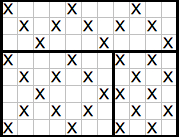
\includegraphics[width=\linewidth,keepaspectratio=true]{doodle/doodle}
\vspace{-9mm}
\end{wrapfigure}

\noindent
When thinking about a hard problem a lot of people like to doodle, to create ``an unfocused drawing that can help the memory and improve abstract thinking''. The most basic form of doodle is a repetitive pattern covering the whole page. One way to create such a pattern is to take a graphing paper and start in the top-left corner $(0,0)$ and fill out the square, then move down and right one square $(1,1)$, fill it out, and so on. Every time you hit the edge of the paper you reverse direction, until you are back at the starting point. This will create a very soothing pattern.

However, to ensure you don't spend the whole competition doodling you need to figure out how how many squares you will have to fill in the paper to complete the doodle before you even start doodling.

\Input
$1 \leq n \leq 4000$\\
The number of testcases\\
For each $n$:\\
$2 \leq x, y \leq 20000$\\
The height and width (in squares) of the graphing paper.
\Output
The number of unique squares you will have filled in before you are done with your doodle.

\Xample{doodle/doodle}

